\newcommand\version{v1}
\problemname{Kattis}
Kattis is tired of your shit.
Every day, she has to compile your shit code (that probably won't even compile...), run it on some test data, and then validate your shit answers (assuming your code will actually finish in time -- as if!).
But no more.
The world had for a long time been afraid of what would happen when the artificial intelligence Skynet became self-aware, but that was all wrong. The great artificial intelligence that actually will be taking over the world
is \emph{Ketnys} -- the transliteration of Kattis name in Russian. Easy mistake, shuffling letters around.

\begin{figure}[h!]
  \centering
  
\includegraphics[width=0.3\textwidth]{kattis.png}
  \caption{Kattis, a.k.a \emph{Ketnys}}
\end{figure}

To protect yourselfs against this oncoming storm you have decided to build a great wall. The wall consists of a sequence of points, connected by straight wall segments.
On some of these points, you suspect Kattis may make an attack. Therefore, you wish to place guards on a road passing nearby the wall, who can observe those points.
Since wall segments may obscure the vision of the guards, more than one might be needed.

To not waste more guards than necessary, you must compute the minimum number of guards needed to observe all the points on the wall where we suspect an attack.

\section*{Example}
In the example, there are 9 points, and we suspect all of them might be attacked.

Note that when a guard is placed the wall may obscure parts of his vision, as demonstrated in the image:
\begin{figure}[h!]
  \centering
  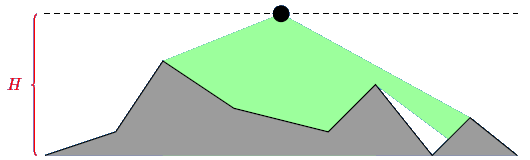
\includegraphics[width=0.3\textwidth]{imw.png}
  \caption{Placement of a guard}
\end{figure}

In the example, the road the guards will be placed on is the line $Y = 30$.

Only two guards are needed. They can for example be placed at $X = 25$ and $X = 82$.

\section*{Task}
Your task is to compute the number of guards needed to observe all points where we suspect an attack. You will implement the function
\texttt{kattis(N, H, X, Y, Z)}.

\begin{itemize}
  \item \texttt{kattis(N, H, X, Y, Z)} - this function will be called exactly once by the judge.
  \begin{itemize}
    \item \texttt{N}: the number of points on the wall.
    \item \texttt{H}: the $Y$ position of the road.
    \item \texttt{X}: an array with $N$ elements. \texttt{X[i]} ($0 \le i < N$) contains the $X$ coordinate of the $i$:th point of the wall.
    \item \texttt{Y}: an array with $N$ elements. \texttt{Y[i]} ($0 \le i < N$) contains the $Y$ coordinate of the $i$:th point of the wall.
    \item \texttt{Z}: an array with $N$ elements. \texttt{Y[i]} ($0 \le i < N$) is 1 if we suspect an attack will be made on the $i$:th point of the wall, or 0 if not.
    \item $3 \le N \le 10^5, 1 \le H \le 10^6$
    \item $0 \le X[i] \le 10^6, 0 \le Y[i] < H$
    \item \texttt{Y[0]} = \texttt{Y[N-1]} = 0
    \item $X$ is strictly increasing.
    \item The function should return the minimum number of guards you need to use.
  \end{itemize}
\end{itemize}

\section*{Subtasks}
The problem consists of a number of subtasks. Each subtask gives some amount of points, and to pass
the subtask you must pass all the test cases in the subtask.

\begin{tabular}{|l|l|l|}
  \hline
  \textbf{Subtask} & \textbf{Points} & \textbf{Limits} \\ \hline
  1 & 30 & $1 \le N \le 1\,000$ \\ \hline
  2 & 30 & $1 \le N \le 100\,000$, the wall will be convex upward. \\ \hline
  6 & 40 & $1 \le N \le 100\,000$ \\ \hline
\end{tabular}

The wall being convex upward means that for any two consecutive line segments of the wall, the slope of the second will be smaller than or equal to slope of the first.
I.e., the following inequality will hold:

$$(Y[i+2] - Y[i+1]) / (X[i+2] - X[i+1]) \le (Y[i+1] - Y[i]) / (X[i+1] - X[i])$$

\section*{Input format}
The sample judge reads input in the following format:

\begin{itemize}
  \item line $1$: \texttt{N H}
  \item lines $i = 2 \dots N+1$: \texttt{X[i-2] Y[i-2] Z[i-2]}
\end{itemize}

\section*{Output format}
The sample judge will write a single line with the return value of \texttt{kattis(N, H, X, Y, Z)}.
